\documentclass[]{final_report}
\usepackage{graphicx}
\usepackage{hyperref}

\def\studentname{Luke Sell}
\def\reportyear{2022}
\def\projecttitle{Metaheuristics}
\def\supervisorname{Eduard Eiben}
\def\degree{MSci (Hons) in Computer Science}
\def\fullOrHalfUnit{Full Unit}
\def\finalOrInterim{Final}

\begin{document}
\maketitle

\chapter*{Declaration}

This report has been prepared on the basis of my own work. Where other published and unpublished source materials have been used, these have been acknowledged.

Word Count: Approximately 12491 words including the Appendix

Student Name: \studentname

Date of Submission: \today

\newpage
\tableofcontents\pdfbookmark[0]{Table of Contents}{toc}
\newpage

\chapter*{Abstract}
\addcontentsline{toc}{chapter}{Abstract}

\section*{Introduction and Background}
\addcontentsline{toc}{section}{Introduction and Background}

A metaheuristic is a general use type of heuristic search algorithm that is able to quickly finding good solutions to a range of optimisation problems by efficiently exploring the search space. In theory it does not use the properties of a specific problem to modify how it searches for a solution, but instead follows a general strategy for all problems. This allows it to be used as a basis for designing algorithms to solve any problem, however it is often the case that once it is implemented, the algorithm is extended to make use of optimisations specific for this problem. Metaheuristics use stochastic, i.e. semi random, searching to counter the combinatorial explosion common in optimisation problems by better covering the search space to find a near optimal solution. In contrast standard heuristics are designed to solve specific problems and are not usable for anything else, but they can be used as part of a hybrid algorithm through combination with a metaheuristic. These both differ from exact methods which always find the optimal solution, but take much longer, such as the well known Branch and Bound algorithm. Metaheuristics are able to work well even without knowing anything about the problem and most importantly are better at escaping from local optima than standard heuristics, through the use of intensification and diversification methods. Metaheuristics are most useful when finding the most optimal solution through an exhaustive search would take too long, e.g. the Travelling Salesman Problem, which is a $NP$ hard problem and has a search space that grows exponentially relative to the size of the problem. There are different types of metaheuristics with varying strategies used to guide the search that each have their own advantages and disadvantages and can be grouped by classifications based on how they search for a solution to a problem. Optimisation problems are classified by how they are structured, they are usually comprised of an objective function to be optimised, variables, variable domains and constraints, e.g. pseudo boolean optimisation problems such as the Knapsack Problem, have a variable domain that is restricted to a boolean value, i.e. zero or one. This was the problem I was originally going to implement for this project, but the Travelling Salesman Problem is the best known optimisation problem with more significance in research material and therefore a better choice. Humans as well as animals have proven to be capable of solving these problems with relative ease, producing near optimal results, providing a basis for comparison as well as inspiration when designing metaheuristics. For example it is thought that humans use the methods of no line crossing and convex hull to solve the Travelling Salesman Problem, by comparing the results of using these methods I can also gauge the success of my own metaheuristics. Indeed many metaheuristics do use physical or biological processes as a basis for their design. Thus metaheuristics clearly provide an alternative way to solve these difficult problems and have yet to be researched in sufficient depth, requiring further investigation that this project will attempt to sufficiently complete within the scope set out previously.

\newpage
\section*{Aims and Objectives}
\addcontentsline{toc}{section}{Aims and Objectives}

The overall aim of this project is to understand the different strategies used by various metaheuristics, to design and implement examples of a subset of these metaheuristics, that cover a range of classifications, to solve the travelling salesman problem and to compare the efficiency of each of them by benchmarking them on several problem instances with differing search parameters, so that they can be tuned and improved. To do this I will have to research these metaheuristics, explain how they work and how I can implement each of them. I will also need to be able to use my implementations through the use of a GUI that allows for each algorithm to be used on a generated problem and for the results to be displayed. Additionally I will need to follow professional software engineering principles in the design and development of my program, such as using a version control system, using the Agile development process, unit testing, design patterns etc. skills which I will gain further experience of during this project and improve my abilities as a software engineer. Finally in writing my reports I will need to critically analyse the material I am reading and how I use it in my project to create a thorough overview of metaheuristics. In extension to this, the program has multiple potential uses of multi threading, e.g. separating the running of metaheuristics from the GUI, I could also implement additional problems to solve to provide further comparisons for the metaheuristics.

\newpage
\section*{Overview of Early Deliverables}
\addcontentsline{toc}{section}{Overview of Early Deliverables}

To begin I will design and implement the Tabu Search Metaheuristic, this will require me to first set up an initial code structure and a basic user interface. I will be writing my code in C++17 and using the SDL 2 library for GUI handling, I will also be using the Catch 2 library as my testing framework. Once the code is implemented, I will have to thoroughly test it on example problems to get a better understanding of how it can be used.

I will need to write reports on computational complexity, Local Search and Tabu Search, this will involve researching these topics using the sources I have found already and describing how they relate to the overall project. Computational complexity will be important in explaining the usefulness of metaheuristics as the problem they will be used on is $NP$ hard, finding the best solution would be infeasible, so understanding this will motivate the use of metaheuristics instead to solve the problem. I will then begin research on the first two metaheuristics and will describe how they work and design the algorithms in pseudocode so that I can implement them later. I will also evaluate their key properties and how this modifies the way they search for a solution, which will be useful later when I need to compare the individual metaheuristics against each other.

\section*{Overview of Final Deliverables}
\addcontentsline{toc}{section}{Overview of Final Deliverables}

I will continue with implementing other metaheuristics and testing them, I could extend this by implementing even more heuristics on other problems in addition to the Travelling Salesman Problem. I will also implement a GUI for the metaheuristics to use them, this will involve using the SDL 2 library. To do this I will first create draft designs of what I expect the GUI to look like, before implementing it and then testing it as a user to make sure it functions properly and intuitively. I will finally benchmark and compare the different metaheuristics by running them several times on different problem instances and recording the times in a log, which I will then use for my comparison.

I will continue my research with reports on Iterated Local Search, Genetic Algorithms, and Memetic Algorithms, this will further my understanding of different types of metaheuristics and allow me to design and implement variations of them and finally benchmark them on example problems for a comparison on the efficiency of each individual metaheuristic.

\chapter*{Theory}
\addcontentsline{toc}{chapter}{Theory}

\section*{Basics of Computational Complexity}
\addcontentsline{toc}{section}{Basics of Computational Complexity}

\subsection*{Expressing Complexity}
\addcontentsline{toc}{subsection}{Expressing Complexity}

Computational Complexity is used to define an algorithms or problems usage of resources, most importantly for metaheuristics, time and memory, which depends on the size of the problem, it is therefore expressed as a function of the size of the input for the algorithm or problem. Different complexity functions are often used, most commonly big $O$ notation, which describes the asymptotic behaviour with an input size approaching infinity by hiding constant factors and smaller terms of $n$, for example $T(2n^{2} + 2)$ would become $O(n^{2})$, which describes the behaviour independent of any specific details of the device and programming language used\cite{barak:2007}. This only describes theoretical cases, in practice the usability of an algorithm might depend on specific details of the implementation. For benchmarking metaheuristics I will use best, worst and average case, as these will give a good estimation of the time taken whatever the problem type, size or instance. Best and worse case describe the behaviour and complexity of an algorithms as it scales in terms of the minimum and maximum times taken for the best and worse inputs of size n respectively. Finally the average case is the time it takes on average, assuming each input is equally likely. Worst case complexity is the most useful as it can be used to guarantee an algorithm will take at most some time, which is important when deciding how to use the algorithm to solve problems, although attempting to find an algorithm that has a best or average case complexity that is significantly better than the worse case can be important if most inputs for the problem are in these cases.

\subsection*{Complexity Classes}
\addcontentsline{toc}{subsection}{Complexity Classes}

A complexity class is as a set of similar problems, defined in terms of reductions, this is proving a problem is at most as difficult as another problem, allowing a problem to be reduced to a problem for which an algorithm to solve it is already known. For this project the factors of significance are classes based on optimisation problems, of note is the class of $NP$ or nondeterministic polynomial time. This is the set of decision problems, problems where the solution is a boolean value corresponding to if there is a valid solution, with solutions that can be verified, but not solved in polynomial time, using a deterministic turing machine, i.e. they can only be solved non deterministically in polynomial time\cite{barak:2007}. $NP$ is therefore the set of all problems that can be solved in $NTIME$, i.e. $O(n^{k})$ or non deterministic time, and is the basis for several other complexity classes, most importantly $NP$ complete and $NP$ hard, which contain the hardest problems in $NP$ and the problems at least as hard as the hardest problems in $NP$ respectively. By contrast the complexity class $P$ is made up of problems that can be solved in polynomial time by a deterministic turing machine and is therefore a subset of $NP$, unfortunately most problems are not in this complexity class and therefore do not have known efficient exact solving algorithms\cite{barak:2007}. Function problems are problems with solutions that provide information about the solution, e.g. the Travelling Salesman Problem, which has solutions comprising of the order in which each city is visited. These problems are in the complexity class $FNP$, which is related to $NP$ in that all function problems can be represented as decision problems, for example deciding if a solution of at least some required quality exists and therefore they have equivalent time complexities\cite{barak:2007}. For such intractable problems it is better to instead search for a solution using a metaheuristic as finding the most optimal solution with certainty may be infeasible given limited resources, whilst a metaheuristic can find a near optimal solution in a significantly shorter time frame.

\newpage
\section*{Optimisation Problems}
\addcontentsline{toc}{section}{Optimisation Problems}

\subsection*{An Overview}
\addcontentsline{toc}{subsection}{An Overview}

Optimisation problems involve finding the most optimal solution to a problem from a search space of solutions, there are many such problems in practice and being able to solve them efficiently would have profound consequences for the world in general. Initially the project aimed to implement a pseudo boolean optimisation problem, like the Knapsack Problem, but upon further research and reflection I have decided to instead focus on the Symmetric Euclidean Travelling Salesman Problem. It is often used as a benchmark for testing algorithms and has real world uses such as in vehicle routing and circuitry, by solving the Travelling Salesman Problem, these similar problems can also be solved using the same algorithm with only minor adaptions.

\subsection*{The Travelling Salesman Problem}
\addcontentsline{toc}{subsection}{The Travelling Salesman Problem}

The Travelling Salesman Problem can be defined as finding the shortest tour going through all cities only once. This is a well known $NP$ hard and $NP$ complete optimisation problem, as it can be reduced to a $SAT$ problem\cite{barak:2007}. It can be expressed as a combinatorial optimisation problem, i.e. a problem with a finite or countably infinite search space, and a brute force attempt to solve it would involve evaluating $\frac{(n - 1)!}{2}$ solutions, $n$ being the number of cities in the problem. Although there are more efficient exact methods known, as the Travelling Salesman Problem is $NP$ hard and assuming $P \neq NP$, no polynomial time algorithm exists to solve it\cite{blum:2001}. As such it is clearly not feasible to find the most optimal solution with certainty, but to instead find a near optimal solution using a metaheuristic.

This problem is a good example of the advantages of using metaheuristics to find solutions in a relatively short time frame, as well as being more complex and representative of real world problems such that I can sufficiently compare the metaheuristics against each other. To express it as an optimisation problem, the Travelling Salesman Problem must have an objective function to evaluate each solution, i.e. the sum of the distances between each city in the tour, a search space of valid solutions, and an instance to describe the current problem, i.e. the matrix of distances between cities. This problem is best represented using permutation encoding to represent the ordering and relationships between cities, meaning all cities appear in the order exactly once. There must also be a set of possible moves from the currently selected solution, this neighbourhood can be constructed in a variety of ways by defining what a neighbour solution is and how limited this definition is.

For the Travelling Salesman Problem a neighbour can be moved to by changing the order in which the cities are visited, this can be achieved by swapping cities adjacent in the tour or those that are further apart, defined as inversion and transposition respectively. These produce neighbourhoods of size roughly $n$ and $n^{2}$ respectively\cite{siarry:2016}. Transposition has better results\cite{siarry:2016} so I am using that as the basis for my implementation of the Travelling Salesman Problem.

The calculation of the quality of a solution should be implemented using the previous solution by considering the modifications made moving to the current solution. This significantly reduces the computational complexity of calculating the cost of a solution from linear time to constant time\cite{siarry:2016}, for example the quality of a solution can be found by subtracting the edges that are removed and adding the edges that replaced them. Finally, it is not necessary to evaluate the quality of all neighbours before selecting a move, instead a limited number can be evaluated to reduce the time taken by the algorithm, this does not reduce the average quality of selected solutions by a significant amount and it is suggested that for the neighbourhood I am using, evaluating a few dozen would be sufficient\cite{siarry:2016}.

It is suggested in \cite{martin:2010} that the theoretical choice to make metaheuristics independent of the problems they solve should be ignored in practice to improve performance, however the algorithm design should try to make sure that these problem dependent implementations be separated from the general metaheuristic. It is also stated in \cite{siarry:2016} that it is impossible to design universal operators for all problems, meaning operators must be defined for each problem. I have therefore chosen to do this by implementing the problem dependent parts inside the problem class itself, as this will allow me to easily add new problems without requiring any changes to the metaheuristics and will also allow me to implement a problem class hierarchy to define what is required to express an optimisation problem.

Additionally the Travelling Salesman Problem has the somewhat unique characteristic among optimisation problems of having its best solutions clustered together, this means that the best solutions are comprised of similar sub orderings of cities, which allows me to make certain assumptions to improve the implementation of the metaheuristics, by searching around these sub orderings to find the globally optimal solution.

Another common method of generating moves is the usage of ejection chains, the best known for the Travelling Salesman Problem is the Lin and Kernighan method, this involves ejecting elements from the solution, thus creating infeasible solutions known as reference structures, then constructing a new solution by adding edges to create a valid tour of cities\cite{siarry:2016}. However I have decided not to implement this method, even though it is suggested to be better, as it would be significantly more complex and the previous method has proved sufficient for problems of the size I am generating for this project.

\newpage
\section*{Local Search}
\addcontentsline{toc}{section}{Local Search}

\subsection*{Hill Climbing}
\addcontentsline{toc}{subsection}{Hill Climbing}

Hill Climbing is the simplest metaheuristic, it involves making small `local' changes to a solution to attempt to improve and replace it, forming a sequence of solutions known as a Markov Chain, because all solutions depend on the previous solution, this is therefore known as a single state or trajectory metaheuristic\cite{siarry:2016}. It continues until the most optimal reachable solution is found, at a `hill', where all possible neighbour solutions are less optimal than the current solution. This implementation is the most basic type of Local Search, as well as being the most limited in its success, it will often get stuck at locally optimal solutions and stop without being able to find a globally optimal solution if that meant first moving to less optimal solutions to reach it.

\begin{figure}[h]
	\centering
	\fboxsep 2mm
	\framebox{
		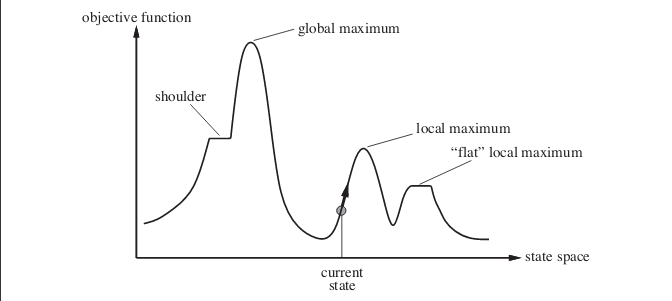
\includegraphics[width=14cm]{optima}
	}
	\caption{\label{fig:optima} A Local Optima}
\end{figure}

Therefore it is necessary to use global optimisation algorithms in almost all practical problem cases. A simple modification to implement a global optimisation algorithm using a Local Search technique is by periodically restarting the algorithm, so that if the Local Search has reached a local optima, the algorithm will restart at a randomly constructed solution and continue. However this is not very effective as selecting a restart location at random will discard knowledge gained during the previous searches, for instance the Travelling Salesman Problem has clusterings of solutions and restarting at a random location will likely move the search outside this region.

Hill Climbing modified from \cite{luke:2013}

\begin{verbatim}
1:  S <- random solution
2:  repeat
3:    R <- neighbour(S)
4:    if Quality(R) > Quality(S)
5:      S <- R
6:  return S
\end{verbatim}

\subsection*{Simulated Annealing}
\addcontentsline{toc}{subsection}{Simulated Annealing}

Other methods of selecting the next solution, known as a `move strategy', exist, such as First Improving and Steepest Ascent\cite{glover:2015}, but the most significant adaption is Simulated Annealing. Simulated Annealing differs in that it selects its next move stochastically, whilst it will still be more likely to select moves that are improving, i.e. moves that decrease the `energy' of a solution, it is able to select worsening moves, allowing it to escape local optima. The basis for Simulated Annealing is the Metropolis Algorithm, which when used as the acceptance rule, always accepts improving moves, otherwise they are only accepted with probability $e^{\frac{\Delta E}{T}}$. Therefore the greater the increase in the `energy' of the solution, the smaller the chance of acceptance is. In addition the greater the `temperature' the more likely a move is to be selected, as the `temperature' of the algorithm is decreased over time, this results in fewer worsening moves being accepted and eventually only improving moves are accepted\cite{siarry:2016}. Therefore the algorithm initially begins as a random walk of the search space and transitions to Hill Climbing over the time the algorithm is run\cite{luke:2013}. Usually the temperature decrease is geometric, i.e. multiplied by a constant factor, resulting in a slow decrease in temperature allows the algorithm to converge to a global optima, whilst a fast decrease from a linear reduction in temperature results in a locally optimal solution.

Simulated Annealing modified from \cite{luke:2013}

\begin{verbatim}
1:  t <- temperature
2:  S <- random solution
3:  Best <- S
4:  repeat
5:    R <- neighbour(S)
6:    if Quality(R) > Quality(S) or p
7:      S <- R
8:    Decrease t
9:    if Quality(S) > Quality(Best)
10:     Best <- S
11: until t <= 0
12: return Best
\end{verbatim}

\newpage
\section*{Tabu Search}
\addcontentsline{toc}{section}{Tabu Search}

Tabu Search introduces the usage of short and long term memory to increase the efficiency of the search, solutions previously visited are `tabu' for an arbitrary amount of time to stop the algorithm returning to them. When these solutions are removed from the tabu list, it allows the algorithm to revisit them and select neighbours that were not selected previously, a larger tabu list results in a wider search, allowing the algorithm to escape cycles around local optima and move into unexplored regions. In \cite{glover:1999} it is suggested that memory usage can be categorised into four dimensions, to consider the quality, influence, recency, and frequency of solutions, to better understand how to progress the search. Intensification and diversification rules are used to direct the search into more promising and entirely new regions respectively. This usage of memory instead of a stochastic search makes Tabu Search a deterministic algorithm in theory, although in practice in might be the case that only a subset of neighbours are explored, or the search may be implemented as part of a hybrid metaheuristic. A candidate list of solutions can also be used for selecting the next move, allowing greater influence in selecting the available neighbours, although a random candidate list can be used instead and is sufficiently effective.

The importance of using additional forms of intensification and diversification is suggested\cite{siarry:2016}, however the minimalistic Tabu Search already provides exceptional results for the Travelling Salesman Problem and a more complicated algorithm would be increasingly difficult to tune, as such a brief overview will be able to cover the advantages of implementing these additions sufficiently. The search can be intensified by more thoroughly exploring the neighbourhood of the best solutions found so far, through using a shorter tabu list temporarily, better solutions can be found by revaluating recently visited solutions and selecting different moves from the candidate list. The search could also prefer moves that have been found to improve solutions previously, such as specific orderings of cities in the Travelling Salesman Problem. Diversification can be achieved by jumping to other solutions in the search space, outside the current region being explored, by more significantly modifying the solution. Through using memory to remember attributes of previous solutions and from this calculating which regions have not been explored recently, a solution with differing attributes can be constructed that will direct the search into an unexplored region, this will prevent the algorithm searching a specific region excessively. Aspiration rules can be used to allow moves that are already on the tabu list if certain conditions are met, such as the solution being of a more optimal value, allowing neighbourhoods to be better explored, so that the search can continue even if many moves are on the tabu list\cite{siarry:2016}, which is common when attributes are remembered instead of complete solutions, where unvisited solutions are sometimes considered tabu. Remembering complete solutions in the tabu list is often worse according to \cite{glover:1999}, as more memory is required by the algorithm, although it is used in some cases, such as for remembering `elite' solutions to use in intensifying the search. The algorithm can be further optimised by using hash tables to efficiently access solutions in the tabu list. An adaptive tabu list size is often used, through increasing or decreasing the size periodically, the search can escape cycles seen when moving to solutions recently removed from the tabu list, by considering these moves tabu for longer the cycle can be interrupted, allowing other moves to be selected\cite{siarry:2016}. Another method used is to penalise some moves, instead of these moves being considered tabu, they have a decreased probability of being selected, allowing for greater influence in selecting a move, e.g. by penalising a move frequently selected, instead of forbidding it completely\cite{siarry:2016}.

\newpage
Tabu Search modified from \cite{luke:2013}

\begin{verbatim}
1:  S <- random solution
2:  Best <- S
3:  L <- {}
4:  repeat
5:    Remove from L all > l
6:    R <- neighbour(S, L)
7:    for n - 1 times
8:      W <- neighbour(S, L)
9:      if Quality(W) > Quality(R)
10:       R <- W
11:   S <- R
12:   L <- L and S
13:   if Quality(S) > Quality(Best)
14:     Best <- S
15: return Best
\end{verbatim}

\newpage
\section*{Iterated Local Search}
\addcontentsline{toc}{section}{Iterated Local Search}

Iterated Local Search uses restarts to efficiently explore the search space, by sufficiently perturbing the local optima found in the previous search, a starting solution can be constructed that is outside its influence, but instead in the influence of a nearby local optima, eventually resulting in a sequence of locally optimal solutions being found. Using this method reduces the time required to find a local optima in comparison to random restarts, as the best solutions are commonly clustered together.

\begin{figure}[h]
	\centering
	\fboxsep 2mm
	\framebox{
		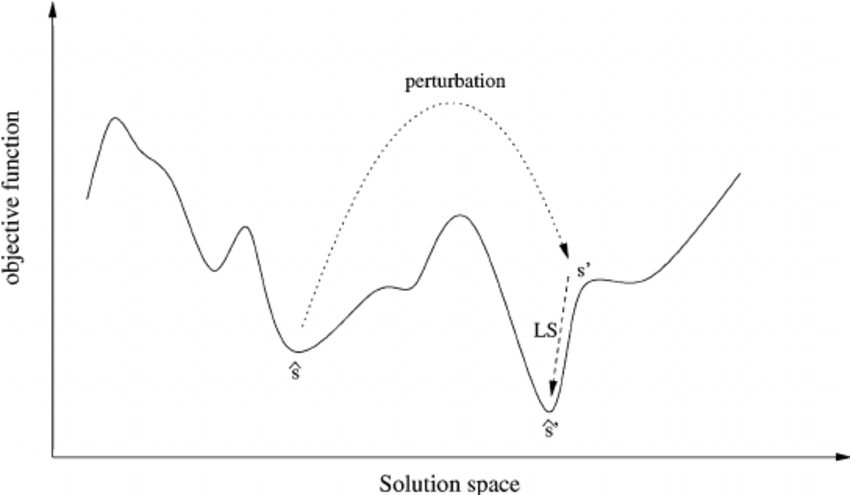
\includegraphics[width=14cm]{ils}
	}
	\caption{\label{fig:ils} Iterated Local Search}
\end{figure}

A `home' solution is often used, to provide a solution to perturb each restart, the home solution is usually the previous local optima found, but adaptations can be made to further influence the direction of the search, through frequently updating the current `home' solution, the search space can be explored more efficiently than through random restarts\cite{luke:2013}. I have implemented this such that only improving solutions are selected as the new home, but stochastic methods can also be used. As the perturbation should result in the Local Search being able to find a different local optima, there should be a significant modification made to the `home' solution, although it should not be too great as to restart the search outside the clustering of optimal solutions resulting in the equivalent of a random restart\cite{luke:2013}. To do this I apply two consecutive randomly selected moves to the home solution, this is similar to the `Double Bridge Move' suggested in \cite{martin:2010}, which replaces four edges, this is the most common perturbation used for the Travelling Salesman Problem as it is both simple and efficient, resulting in solutions of similar cost being constructed. Using an adaptive perturbation strength can be important in making the algorithm independent of the problem, the strength of the perturbation can be updated if the same local optima is repeatedly found or if the search is too slow.

\newpage
Iterated Local Search modified from \cite{luke:2013}

\begin{verbatim}
1:  S <- random solution
2:  H <- S
3:  Best <- S
4:  repeat
5:    repeat
6:      R <- neighbour(S)
7:      if Quality(R) > Quality(S)
8:        S <- R
9:    if Quality(S) > Quality(Best)
10:     Best <- S
11:   H <- NewHomeBase(H, S)
12:   S <- Perturb(H)
13: return Best
\end{verbatim}

\newpage
\section*{Genetic Algorithms}
\addcontentsline{toc}{section}{Genetic Algorithms}

\subsection*{An Overview}
\addcontentsline{toc}{subsection}{An Overview}

Genetic Algorithms are population based metaheuristics implementing rules inspired by natural selection processes, such as selection, crossover and mutation, and are part of the group of algorithms known as Evolutionary Algorithms. Beginning with a population of multiple solutions, the algorithm progresses by selecting good solutions from the current `generation' and `evolving' these solutions using crossover and mutation to construct the next generation, repeating this iterative process indefinitely. Population based metaheuristics like this also benefit from being able to run in parallel, as the process of generating the next population can be split across several threads since the children are generated independent of each other, unlike single state methods where each solution is dependent on the previously found solution, however Genetic Algorithms are slower sequentially as the quality of all solutions in the population has to be completely calculated each generation.

The initial population is randomly generated, producing a variety of `genes' to be used, allowing the algorithm to find a range of solutions rather than prematurely converging on a single solution, although it could be seeded instead if it is known where the optimal solutions are most likely to be found. The size of the population is therefore important to the success of the algorithm and should be large enough to represent the size of the problems search space, but not too large that it increase the time and memory required to complete the search, usually a search space can be properly represented to a sufficient degree with a population much smaller than the search space size, for the Travelling Salesman Problem with a few dozen cities, I have found a few hundred solutions to be best in achieving good results quickly. A sufficient number of generations must be generated to enable the eventual convergence on a globally optimal solution, otherwise there would still be many sub optimal solutions used in the generation process potentially blocking better solutions being found, though it can also be useful to restart the process with an entirely new population if the population has converged prematurely, only carrying over a limited number of solutions or even just the best solution found so far. For some problems a binary representation is used as an encoding and later converted to a natural representation for evaluation, here the `genotype' is used for the application of variation operators, whilst the `phenotype' is used for calculating the fitness of the individual.

\newpage
\subsection*{Selection}
\addcontentsline{toc}{subsection}{Selection}

Selection is used to choose the solutions that will be parents to construct the next generation through crossover, a solution can be selected for this purpose any number of times or not at all, in the Genetic Algorithm the children that are generated completely replace the parents in the next generation. There are several methods of implementing this in practice, but they are all stochastic, being more likely to select better individuals, but still allowing the selection of worse individuals to maintain genetic diversity and reduce the probability of some solutions being repeatedly selected, although if the selection pressure is too low there is genetic drift instead\cite{siarry:2016}. It is therefore important to tune the selection pressure to increase the probability of finding the optimal solution. After the metaheuristic has finished it can be useful to apply a Local Search to the best solution found, this is likely produce an improved solution due to the difficulty population based methods have in constructing locally optimal solutions. Proportional Selection was initially used by Genetic Algorithms, this involves selecting individuals with a probability proportional to the fitness of the solution, however as the algorithm converges and many solutions are similar in fitness all have near equal probabilities of being selected resulting in genetic drift, this requires the scaling of solutions relative to each other, increasing the complexity of the selection process. Therefore Tournament Selection is usually considered the best selection operator due to its simplicity and is therefore the one I have chosen to implement, it involves holding `tournaments' to select the parents, the best individuals `win' and are selected for crossover, but only a subset of the population takes part, usually two\cite{luke:2013}. However I have had more success in using a higher tournament size to increase the selection pressure, to more quickly converge the population and thus decrease the time taken by the algorithm, as I need to ensure the metaheuristic will run on a variety of devices.

Tournament Selection modified from \cite{luke:2013}

\begin{verbatim}
1:  P <- population
2:  t <- tournament size
3:  Best <- random individual
4:  for i from 2 to t
5:    Next <- random individual
6:    if Fitness(Next) > Fitness(Best)
7:      Best <- Next
8:  return Best
\end{verbatim}

\newpage
\subsection*{Crossover}
\addcontentsline{toc}{subsection}{Crossover}

Crossover involves `reproducing' two or more parent solutions to produce children, parts of each parent are used to construct the children, for problems with binary representations this is relatively simple, all that is required is to swap a number of individual genes between the parents. In practice this means that the value of the bit in one parent becomes the value of the bit in the same position of the other parent and vice versa. This happens several times resulting in children that are substantially different from either parent used to construct them. There are several methods used to select the bits to swap, the most successful is selecting the bits at random, known as uniform crossover, which I have used, but one and two point crossover are also used by only swapping bits between selected points in the genotype.

\begin{figure}[h]
	\centering
	\fboxsep 2mm
	\framebox{
		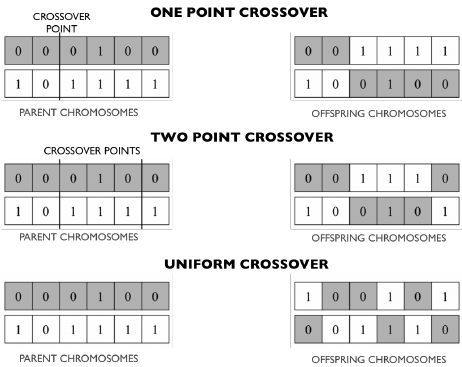
\includegraphics[width=14cm]{crossover}
	}
	\caption{\label{fig:crossover} Crossover}
\end{figure}

Implementing this for the Travelling Salesman Problem is more difficult as it is usually expressed using permutation encoding, the order in which the cities are visited, using these methods without modification would not be efficient at constructing good solutions. For permutation encoding it is more important to consider the sub orderings of the cities instead of the individual position of the cities in the order\cite{siarry:2016}, crossover should therefore maintain these sub orderings to be used successfully. This involves no actual swapping between the parents, but instead reordering select cities to match the order that they follow in the other parent. However crossover is not able to construct every solution in the search space, only those that can be constructed from the current population, therefore another operator is required to introduce genetic diversity, through mutating solutions\cite{luke:2013}.

\subsection*{Mutation}
\addcontentsline{toc}{subsection}{Mutation}

Mutation is used to introduce new genes into the population, allowing all solutions to be constructed, this is similar to Local Search, as such I have implemented this by replacing the solution with a random neighbour. In the Genetic Algorithm the mutation rate is usually low, with most children constructed from crossover. I did not implement this completely, but instead perform crossover for constructing all children, then applying a small mutation to each of them, although mutation can be destructive for some optimisation problems, for the Travelling Salesman Problem it is fine to mutate all individuals. Finally there are different termination criteria that can be used, I have used the number of generations, however perhaps a better method would be to terminate the search if a generation does not improve on the previous generation, or if it is clear the population has converged, i.e. the variation in fitness of the population is very low.

\subsection*{Modifications}
\addcontentsline{toc}{subsection}{Modifications}

It is possible to use the variation operators stochastically by tuning the probability that an operator is applied if at all, this could mean only mutating a few solutions, the probability can also be modified during the search, although it is important to always have a mix of crossover and mutation. Another issue becomes apparent if the parents used in crossover are too similar, this will not produce sufficiently different children and if the entire population is the same, the search has converged, the probability of this occurring can be reduced by not allowing crossover between similar parents or by introducing new random solutions into the population if there is not sufficient genetic diversity in the current population. Elitism methods can also be used, by selecting the best solutions in a generation to be part of the next generation without performing crossover or mutation on them, the best solution in a generation will therefore always improve in fitness in successive generations and can be used to construct further solutions through crossover and mutation. This means that the next generation does not completely replace the previous generation, as was the case for genetic algorithms, other Evolutionary Algorithms already use a replacement operator by stochastically replacing the population of parents with children\cite{glover:2015}. However using excessive elitism can cause premature convergence, by over exploiting some regions rather than exploring new regions in the search space\cite{siarry:2016}.

The Genetic Algorithm modified from \cite{luke:2013}

\begin{verbatim}
1:  popsize <- population size
2:  P <- {}
3:  for popsize times
4:    P <- P and {new random individual}
5:  Best <- Pi
6:  repeat
7:    for each individual Pi in P
8:      if Fitness(Pi) > Fitness(Best)
9:        Best <- Pi
10:   Q <- {}
11:   for popsize / 2 times do
12:     Parent Pa <- Select(P)
13:     Parent Pb <- Select(P)
14:     Children Ca, Cb <- Crossover(Pa, Pb)
15:     Q <- Q and {Mutate(Ca), Mutate(Cb)}
16:   P <- Q
17: return Best
\end{verbatim}

\newpage
\section*{Memetic Algorithms}
\addcontentsline{toc}{section}{Memetic Algorithms}

Memetic Algorithms are an extension of the processes used in Genetic Algorithms through the addition of a local improvement operator, producing a hybrid algorithm that uses aspects of multiple metaheuristics, other hybrid metaheuristics exist, but Memetic Algorithms are the most common. Evolutionary Algorithms struggle to converge on optima, they succeed at finding a range of good solutions, but do not Hill Climb like single state metaheuristics, through using a Memetic Algorithm the advantages of both can be implemented. The local improvement operator can be used in a similar way to other operators, it can be used anywhere or even multiple times in the process of constructing the next generation\cite{cotta:2004}. \cite{glover:2015} suggests that pure Evolutionary Algorithms are rare in practice due to their inability to reach optima efficiently and thus most use a form of local improvement. Hybrid algorithms like these are usually superior and I have noticed similar advantages in my implementations on larger problem instances especially.

The Memetic Algorithm modified from \cite{luke:2013}

\begin{verbatim}
1:  P <- Population
2:  Best <- Pi
3:  repeat
4:    for each individual Pi in P
5:      Pi <- Hill-Climb(Pi)
6:      if Fitness(Pi) > Fitness(Best)
7:        Best <- Pi
8:    P <- Join(P, Breed(P))
9:  return Best
\end{verbatim}

\chapter*{Technical}
\addcontentsline{toc}{chapter}{Technical}

\section*{Comparing the Metaheuristics}
\addcontentsline{toc}{section}{Comparing the Metaheuristics}

To implement an efficient and useful metaheuristic it was necessary for me to understand the results they produce and to compare them against each other so that I could both improve the implementations as well as evaluate which metaheuristic was best in the context of the Travelling Salesman Problem. To do this I ran each metaheuristic on the same problem instance, I then repeated this process on several more newly generated problems to provide a sufficient sample size and produce a range of results independent of specific problem instances. From this I was able to record the costs of solutions found and the times required to find them by each metaheuristic.

\begin{verbatim}
Tabu Search
Min Cost: 4943p  | Avg Cost: 5261p   | Max Cost: 5506p
Min Time: 1793ms | Avg Time: 1818ms  | Max Time: 1857ms

Iterated Local Search
Min Cost: 4881p  | Avg Cost: 5365p   | Max Cost: 5823p
Min Time: 2730ms | Avg Time: 2766ms  | Max Time: 2817ms

Genetic Algorithm
Min Cost: 5402p  | Avg Cost: 5997p   | Max Cost: 6560p
Min Time: 1875ms | Avg Time: 1898ms  | Max Time: 1929ms

Memetic Algorithm
Min Cost: 4763p  | Avg Cost: 5326p   | Max Cost: 6369p
Min Time: 6843ms | Avg Time: 13405ms | Max Time: 15492ms
\end{verbatim}

These benchmarks were similar to previous benchmarks I did during the tuning of the parameters and provide an interesting insight into the performance of the metaheuristics. Most surprising are the benchmarks for the Mememtic Algorithm, this has been an efficient metaheuristic on larger problem instances, however on the problem sizes I am attempting to solve for this project, it is significantly slower than the other metaheuristics for little improvement in results. This is clearly due to the increased time used applying the local improvement operator on each solution in the population, as well as the inefficiencies of the population based methods in general. In practice population based methods are easier to multithread with more significant time gains than trajectory methods. The Memetic Algorithm did however provide a significant improvement over the Genetic Algorithm in its ability to find the best solutions. The population based methods had the greatest variation between the minimum and maximum costs of the solutions found, supporting the theory that the initial population generated has a significant impact on the successfulness of the metaheuristic, as well as worse maximum costs in general, likely due to their inability to converge on optima reliably. Iterated Local Search found a reasonable compromise between times and costs, providing significantly better results than the genetic algorithm, but being slightly slower. Overall the best metaheuristic was clearly Tabu Search, despite the simplicity of my implementation, it performed strongly, its maximum time was faster than the other metaheuristics minimum times, whilst providing the best costs on average.

Further extending and tuning these metaheuristics surely would have continued to improve the results even more, but I was able to achieve the best results possible within the scope of the project. I could have extended the intensification and diversification rules used by the Tabu Search for instance, ultimately the population based methods likely had the most to improve, through multithreading, tuning the crossover and mutation rates and using elitism. I likely would have seen better results, but these extensions would have increased the complexity of the implementations further. I would have liked to have ran more benchmarks of the differing modifications and to display the results in a more understandable graph format, but this would have taken a significant amount of time as is clear from the running times of the metaheuristics. It was unfortunately not possible to tune the metaheuristics using smaller problem sizes as these produced wildly differing results. This would justify the use of hyper heuristics to more efficiently tune the metaheuristics, but this would increase the complexity of the project, was not within the scope of the original objectives and would significantly increase the time required to complete the project.

\newpage
\section*{The GUI Design}
\addcontentsline{toc}{section}{The GUI Design}

An important component of an application is its graphic user interface and the user experience it provides, the application must be easily operated by a user so that its functionality can be accessed, I have thus made the interface simple and reactive to the user input, as well as displaying the results in a form that the user can easily understand and view. During this process I drafted designs for the appearance of the GUI, as well as testing the user experience as I implemented it. Through a modular design for the GUI, using the Model View Controller design pattern, I separated the classes for the interaction of each GUI component from the functionality of the metaheuristics, allowing the application to be easily extended to provide new functionalities. I have also used multithreading so that the GUI is not impacted by the response time of the metaheuristics, therefore staying reactive to further user input.

I use the left side of the window to display the results, with the buttons on the right side, I used an appropriate font and layout of GUI components such that it is intuitive for the user, I have also used overlays to indicate when a button is selected, as well as a notification to indicate when sub threads are operating. I could have also used sound effects for additional feedback response, for instance when a button is clicked or results have been returned from a metaheuristic. I would have also liked to have implemented an option to view previous results for the current problem, as well as options for the time given to metaheuristics and the size of the problems generated.

\begin{figure}[h]
	\centering
	\fboxsep 2mm
	\framebox{
		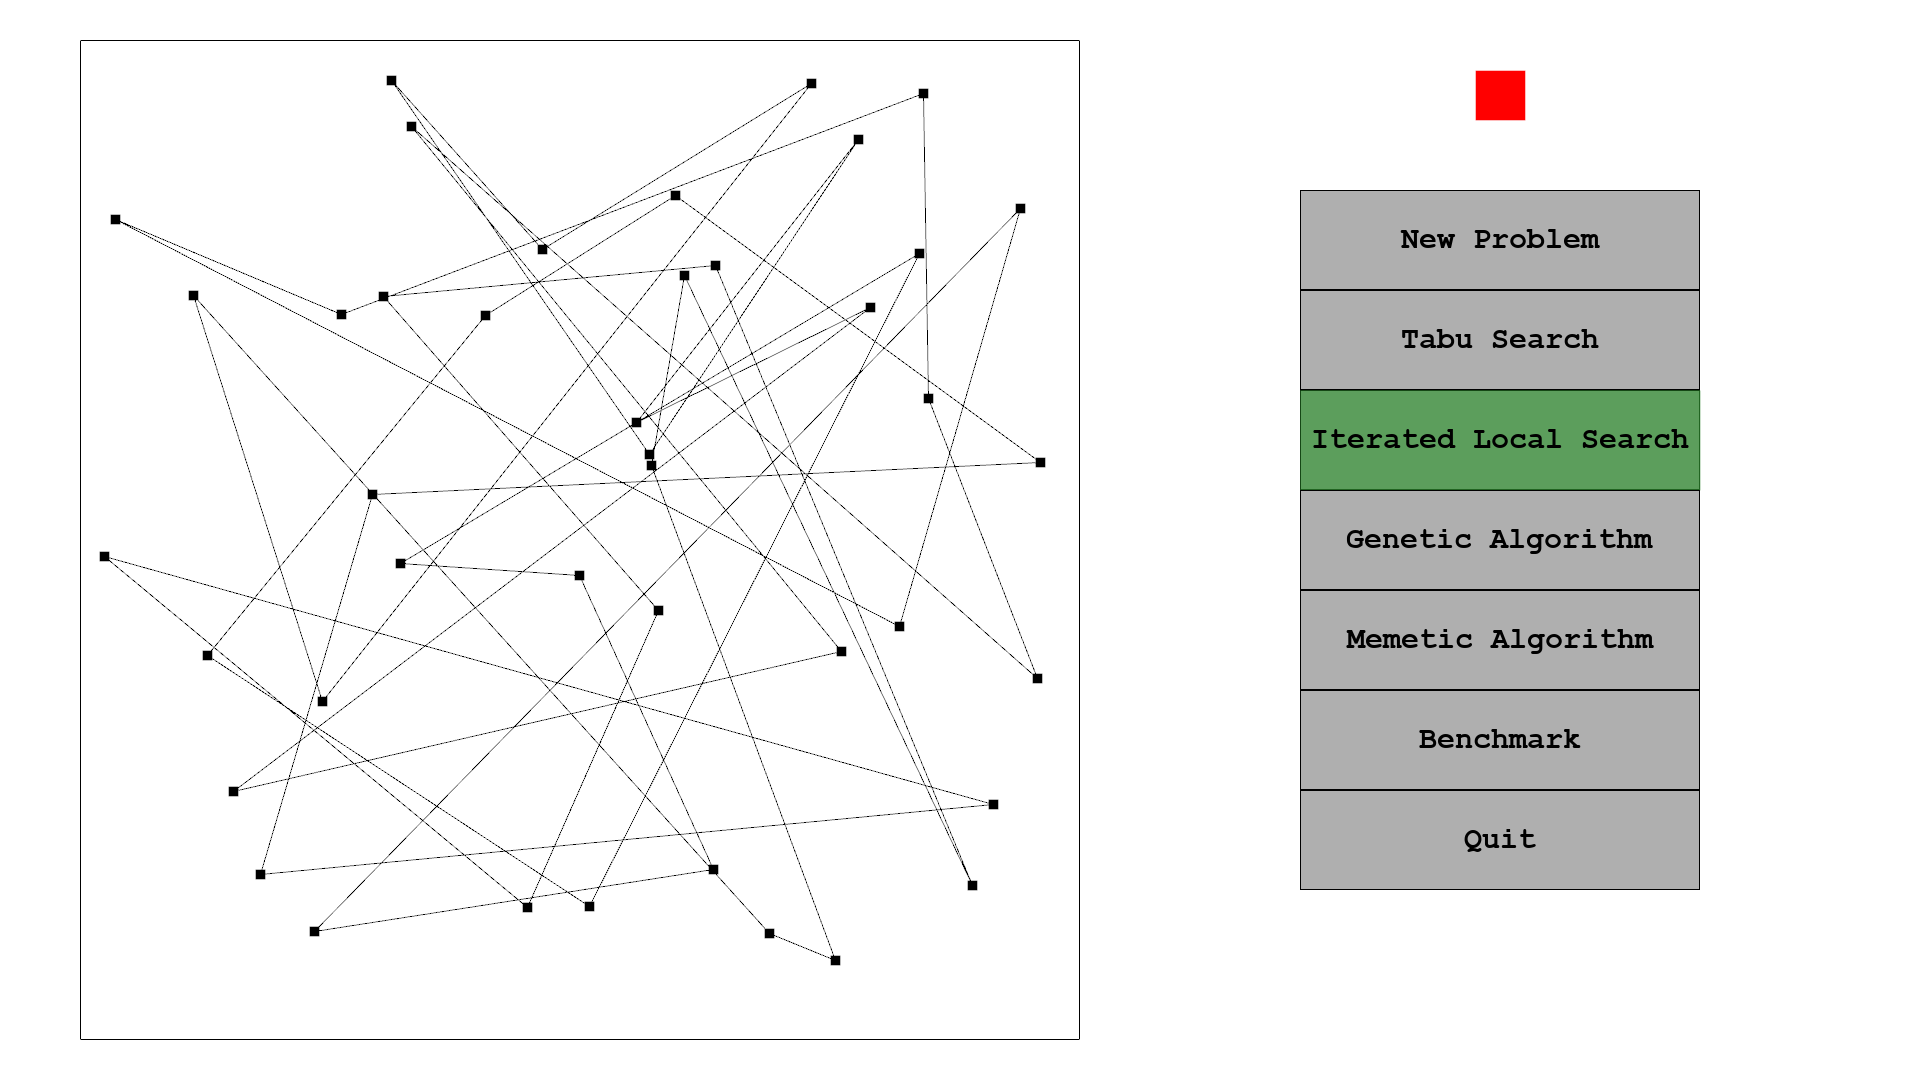
\includegraphics[width=14cm]{gui}
	}
	\caption{\label{fig:gui} The GUI}
\end{figure}

\newpage
Below is an example of a result displayed by the application, clearly this is a near optimal solution that was found using the memetic algorithm, more detailed cost and ordering data is then recorded in the results log once the application has been exited. Although this logging could be improved in its detail, by recording more data about the problem instance, i.e. the cities and their corresponding locations, as well as by displaying this on the GUI.

\begin{figure}[h]
	\centering
	\fboxsep 2mm
	\framebox{
		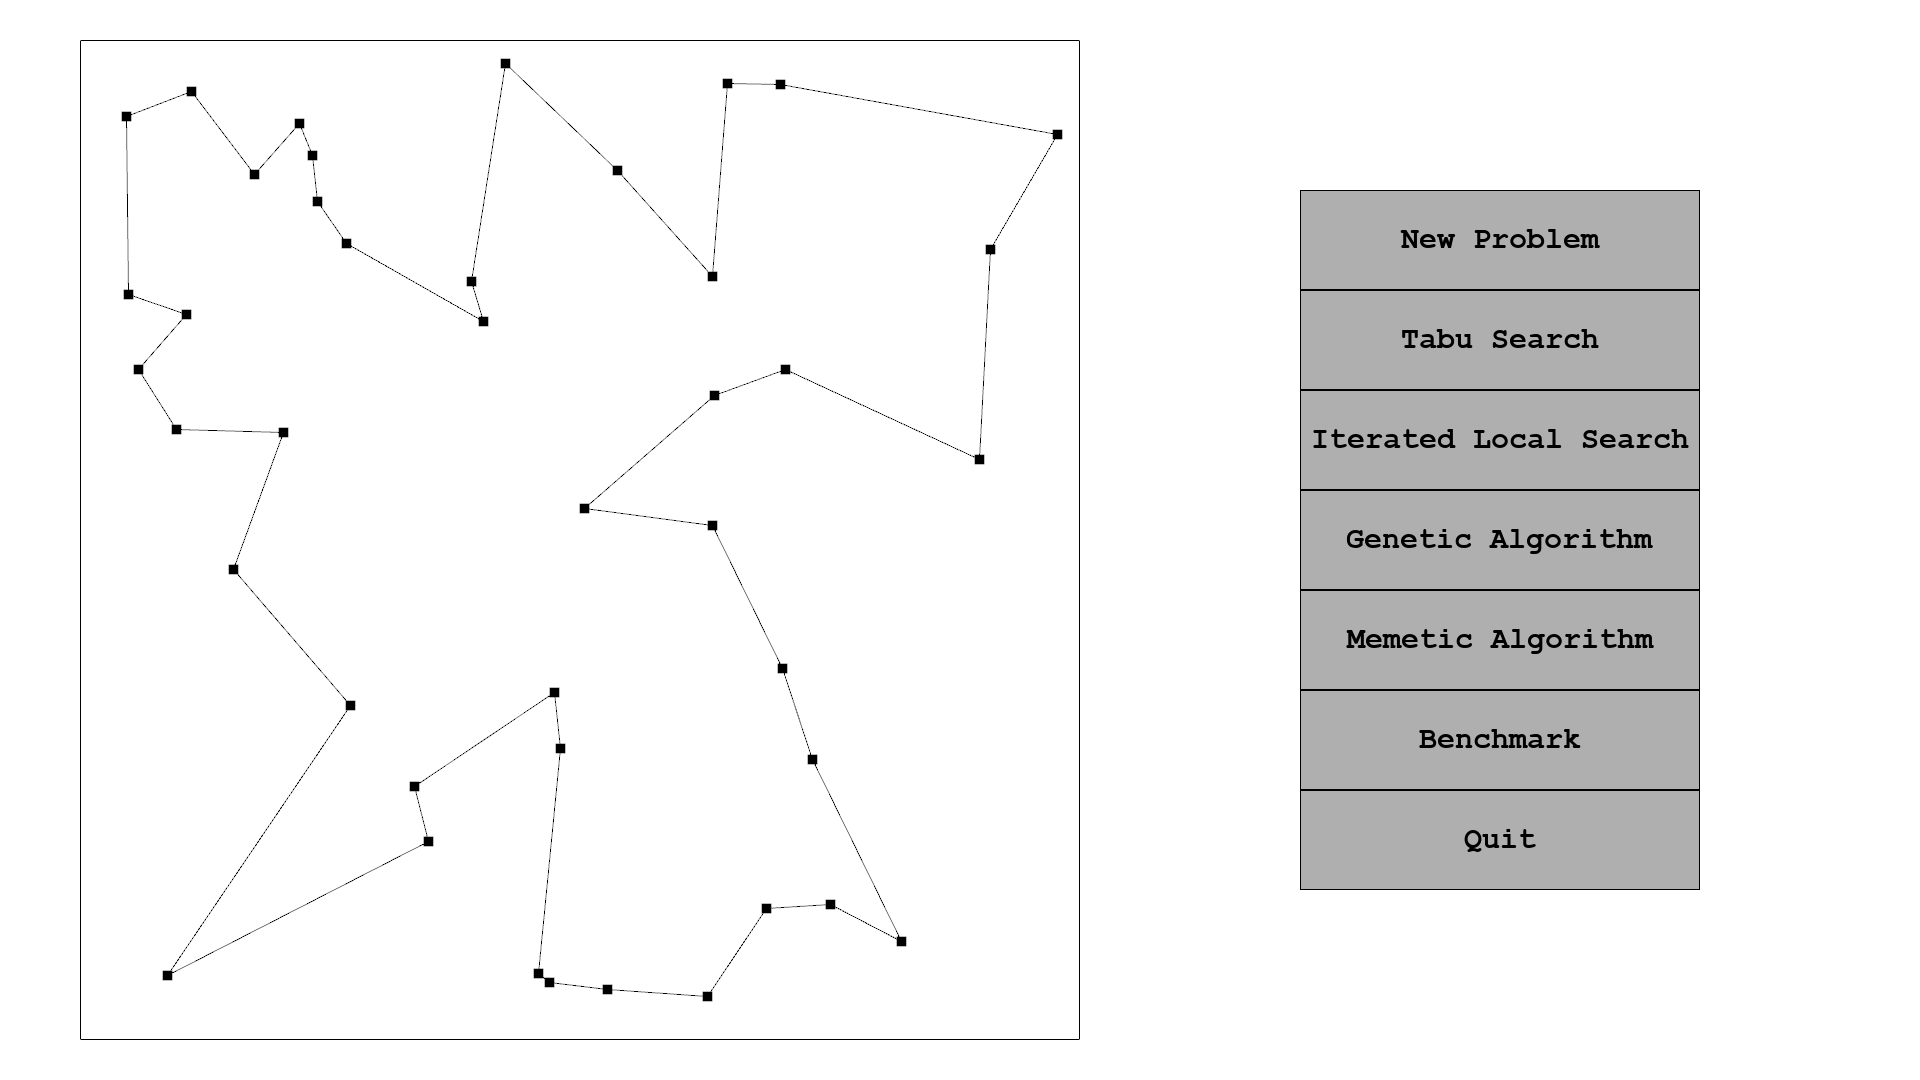
\includegraphics[width=14cm]{tsp}
	}
	\caption{\label{fig:tsp} Displaying a Result}
\end{figure}

\chapter*{Literature Review}
\addcontentsline{toc}{chapter}{Literature Review}

To write my report and research the required background theory I used several sources of differing subjects, some have been integral to the success of the project, whilst others have only been useful in furthering my understanding of metaheuristics in some contexts.

Metaheuristics First Edition 2016\cite{siarry:2016} is a book by leading researchers in the field and covers most metaheuristics, it is the main background theory source for this project, going into significant detail, even beyond the scope of this project. It has been extremely useful in gaining an understanding of metaheuristics and as such has been cited in my report frequently. It suggested a number of optimisations that I used to implement my trajectory metaheuristics to great success, whilst also providing some suggestions on tuning parameters for the metaheuristics. It also provided detailed information on potential modifications for the Travelling Salesman Problem, most notably for implementing crossover efficiently, as well as improving the performance of cost calculations for trajectory moves and how to best implement tabu moves.

Essentials of Metaheuristics Second Edition 2013\cite{luke:2013} is a book covering mostly the implementation of metaheuristics and is therefore the main practical source for this project, it provided inspiration for the pseudocode of every metaheuristic I implemented and as such is the basis for a significant part of the application. However I needed to significantly modify the suggested implementations to improve the performance of the metaheuristics, with this book not providing any useful suggestions on specific modifications for the Travelling Salesman Problem, instead only solving simplistic optimisation problems, but nonetheless provided a good start for my project.

Metaheuristics in Combinatorial Optimization: Overview and Conceptual Comparison 2001\cite{blum:2001} is a research paper providing a good overview of each of the metaheuristics and was used in addition to my main theory source to support my research.

Metaheuristics 2015\cite{glover:2015} is a research paper providing a brief overview of metaheuristics in general and has only been somewhat useful for this project.

Tabu Search Part I 1999\cite{glover:1999} is a research paper by leading researchers in the sub field of Tabu Search, it has been extremely useful in the context of this section of my report and provides sufficient detail for the scope of this project, whilst also suggesting ideas for potential extensions to the implementation of this metaheuristic.

Iterated Local Search: Framework and Applications 2010\cite{martin:2010} is a research paper by leading researchers in the sub field of Iterated Local Search, it has been useful in understanding the metaheuristic and its advantages, as well as the use of metaheuristics in practice.

Memetic Algorithms 2004\cite{cotta:2004} is a research paper by leading researchers in the sub field of Memetic Algorithms, it has been useful in understanding how to combine metaheuristics to construct hybrid algorithms.

Computational Complexity: A Modern Approach 2007\cite{barak:2007} is a book of lecture notes covering computational complexity, it goes into detail beyond the scope of this project, but has been useful in understanding computational complexity in the context of metaheuristics and optimisation problems.

\chapter*{Software Engineering and Development}
\addcontentsline{toc}{chapter}{Software Engineering and Development}

Developing a large and complex application has required me to use many software engineering skills, considering many aspects of the design process, these techniques have allowed me to build a professional, understandable and maintainable program that is able to perform a number of functionalities required by the projects specifications.

I frequently used design patterns to improve my code, both originally and by refactoring, resulting in simpler code. Most notably I used the Adapter and Facade design patterns in the metaheuristic class to encapsulate all interactions with the optimisation problem here, with each individual metaheuristic using the interface, thus reducing the overall complexity and coupling significantly, whilst increasing the cohesion of each class. I also used the Chain of Responsibility and State design patterns for the GUI, for instance the application renders the screen, which then renders the buttons, thus giving each component the option to render additional components. The State design pattern is used to set the active screen, allowing the functionality to change without introducing complex code to handle this. I also implemented the application class as a Singleton with only a single instance, allowing greater control over interactions with it, notably being used statically without requiring global variables, which was necessary for interacting with important rendering and font members for GUI classes, although this could have been improved to reduce coupling. I could have used the Flyweight and Prototype design patterns for GUI components, by using flyweights I could store generic GUI textures to reduce memory usage, and by using prototypes I could clone components to simplify the process of constructing the GUI, other design patterns that are important in this context are the Factory and Builder design patterns.

I also used profilers to improve the performance of my code, this allowed me to see the code that was most active so I could optimise it. I found that a significant amount of time was used to render the Travelling Salesman Problem display, this was due to the application constructing a new GUI texture each frame update. I could have improved this by instead storing the texture representing the currently displayed problem and only updating the texture when required, for instance when a new problem is generated or a result is returned by a metaheuristic. Ultimately I did not do this as the time wasted was not significant and the main thread was only used for handling the GUI.

I used various differing data structures and containers in my code, most commonly Standard Template Library vectors to store lists and doubly ended queues in crossover to simplify reodering. I could have improved my implementation of the Travelling Salesman Problem by using a specialised matrix container, this would have improved the efficiency of indexing elements and allowed additional functionality. I made frequent use of inheritance and composition in my program to represent the class hierarchy, this could have been improved further by refactoring the problem class to instead have a hierarchy of optimisation problems, allowing me to quickly implement optimisation problems in extension to the Travelling Salesman Problem, without modifying how they interact with each metaheuristic.

I also used code styling to ensure my code was easy to understand, through following the Google standard, which is the most popular and thus recognisable to other software developers. To increase my productivity I used the Code Blocks IDE, it provides many plugins and tools that made the process of developing the application easier, such as for code styling and documentation. Additionally I used a version control system through a GitHub repository, to provide the ability to work with other software developers, being able to revert commits and use branches for instance.

For this project I used the Agile development process, with assigning tasks for sprints to implement functionality of the application in vertical slices and release candidates for testing. This was important for completing the initial application for the interim review, as well as implementing and testing new functionality.

Although I was not able to complete unit testing due to issues with the framework I was using, it is nonetheless important to use test driven development in writing unit tests to ensure the program functions as expected and does not regress after refactoring, but to also understand how to implement functionality through the process of extending it iteratively. Necessary for completing this is through the use of a tool for understanding test coverage to ensure the code is fully tested, as well as ensuring edge cases are considered.

\chapter*{Professional Issues}
\addcontentsline{toc}{chapter}{Professional Issues}

\section*{An Overview}
\addcontentsline{toc}{section}{An Overview}

During the development of my program I encountered many potential professional issues regarding the use of third party libraries in the context of licencing and compatibility, these issues greatly impacted the design process and as a result have required me to learn how to properly address them with the professional usage of libraries. At the completion of my project I had already used several libraries for handling user interaction, as well as for unit testing and for documentation. The usage of the SDL 2 library was the most problematic, it was fundamental to my ability to be able to design a professional and modern application that can be ported to any device. However I need to understand what my usage of the library means for the licencing of the program and how to correctly interface with the predominately C code the library uses. There were many compatibility issues that needed to be addressed in the development of the program, whilst still following the software engineering principles I set out for myself at the beginning of the project.

\section*{Licencing}
\addcontentsline{toc}{section}{Licencing}

When developing a professional application it is important to consider the licencing, it would be unethical to use third party libraries without adhering to their licences and would lead to issues regarding the legality of the program. To address this issue I have only used third party libraries with licences that allow for flexibility in developing an application without requirements. Open source software like this has become more common in recent years, allowing many applications to be successfully developed and released to users. By reusing code in the form of frameworks, without the need for developing such code again, which would require a significant amount of time, as well as understanding of, in some cases, complex hardware and software, which is clearly infeasible for small development teams, the development process is simplified significantly. I have myself chosen to use the MIT licence for my application, this is a commonly used licence for research projects and provides a basic licence for my application to safeguard its usage, thus giving me a greater understanding of the implications of licencing and its importance when developing applications.

\section*{Compatibility}
\addcontentsline{toc}{section}{Compatibility}

Usage of third party libraries also has the additional constraint of needing to understand the interface to the libraries functionality. There is commonly documentation, providing details of the interface the software developer can use to interact with the functionality provided by the library, this results in significant amounts of code using the interface. Issues within the library need to be addressed properly, open source software does enable contribution to the development of the library itself, however this might not be realistic and it would be unprofessional to fix these issues by directly modifying internal library code. Instead an adapter should be used for interfacing with the library, this ensures it is clear to future maintainers of the code what the program does, without requiring advanced knowledge of internal library details. If this was not handled correctly it could cause issues when updating the library to a newer version, or could even invalidate the guarantees the interface and its documentation provide, which could be confusing to other developers and produce difficult to find bugs. I have seen this issue frequently in the development of my program, as SDL 2 was originally developed for the C programming language, it does use many features of C++, for instance it cannot handle smart pointers, references and other new additions in C++. This complicated my usage of smart pointers, I needed to provide my own deleters and to pass C pointers to the SDL 2 interface. Other graphics libraries exist for C++ specifically, such as the SFML library, but they are not as popular and do not provide the same level of support for developing in them, thus using the SDL 2 library was the only reasonable option. However despite the issues, this gave me useful experience developing in a commonly used library and addressing the issues surrounding its usage in a professional application so that I can continue to use modern software engineering principles whilst developing.

\chapter*{Conclusion and Self Evaluation}
\addcontentsline{toc}{chapter}{Conclusion and Self Evaluation}

Overall this project has been completely successful in achieving its aims and even extending upon the original objectives. I was able to produce a detailed report describing the theory supporting each of the metaheuristics and then implement them in practice for a real world problem, the well known Travelling Salesman Problem, with near optimal solutions being found in a reasonable time frame and significantly quicker than the best exact methods known. I have also extended my skills in programming through the use of graphics libraries to construct an interactive GUI, as well as multi threading my application. In addition I gained valuable experience in the development of large applications with the usage of modern software engineering principles, including the use of refactoring and modular design, as well as expanding my knowledge of the C++ standard library to better use the programming language in general, producing the most expansive program I have ever developed. There is also significant potential for extending the project, I could have tested the metaheuristics on larger problem instances if I had the computation time to properly tune the metaheuristics and solve the problems. For this I could have used hyper heuristics, the use of heuristics to tune metaheuristics without the need for complex user tuning. As well as solving real world problem instances like those found on the TSPLIB website. These however were all improvements that were in retrospect not necessary for a project of this scope, the report and program I have completed for this project has overwhelmingly proved the usefulness of metaheuristics in theory and practice, proving that this will continue to be an important research area for the foreseeable future, with many potentially hugely consequential discoveries yet to be made that will allow us to solve the most difficult of problems.

\newpage
\begin{thebibliography}{99}
\addcontentsline{toc}{chapter}{Bibliography}
	
\bibitem{siarry:2016} Metaheuristics First Edition 2016 by Patrick Siarry et al.
	
\bibitem{luke:2013} Essentials of Metaheuristics Second Edition 2013 by Sean Luke
	
\bibitem{blum:2001} Metaheuristics in Combinatorial Optimization: Overview and Conceptual Comparison 2001 by Christian Blum and Andrea Roli and published in the research journal ACM Computing Surveys Volume 35 Number 3 2003 pages 268 to 308
	
\bibitem{glover:2015} Metaheuristics 2015 by Fred Glover and Kenneth Sorensen and published on \url{www.scholarpedia.org/article/Metaheuristics}
	
\bibitem{glover:1999} Tabu Search Part I 1999 by Fred Glover and Manuel Laguna and published in the research journal Informs Journal on Computing
	
\bibitem{martin:2010} Iterated Local Search: Framework and Applications 2010 by Olivier C Martin, Thomas Stutzle and Helena Ramalhinho Lourenco in Handbook of Metaheuristics pages 363 to 397
	
\bibitem{cotta:2004} Memetic Algorithms 2004 by Carlos Cotta, Pablo Moscato and Alexandre Mendes in New Optimization Techniques in Engineering pages 53 to 86
	
\bibitem{barak:2007} Computational Complexity: A Modern Approach 2007 by Sanjeev Arora and Boaz Barak at Princeton University
	
\end{thebibliography}

\chapter*{Appendix}
\addcontentsline{toc}{chapter}{Appendix}

\section*{The Original Timeline}
\addcontentsline{toc}{section}{The Original Timeline}

Report on the basics of computational complexity from 08/10/2021 to 17/10/2021

Report on Local Search from 19/10/2021 to 27/10/2021

Report on Tabu Search from 30/10/2021 to 11/11/2021

Implementation of Tabu Search from 19/11/2021 to 30/11/2021

Interim submission on 03/12/2021

Preparation for presentation from 04/12/2021 to 05/12/2021

Report on Iterated Local Search from 06/12/2021 to 12/12/2021

Report on Genetic Algorithms from 13/12/2021 to 20/12/2021

Report on Memetic Algorithms from 21/12/2021 to 28/12/2021

Draft GUI designs from 29/12/2021 to 30/12/2021

Implementation of GUI from 02/01/2022 to 10/01/2022

Testing of GUI from 11/01/2022 to 12/01/2022

Implementation of Iterated Local Search from 13/01/2022 to 23/01/2022

Implementation of Genetic Algorithm from 25/01/2022 to 04/02/2022

Implementation of Memetic Algorithm from 06/02/2022 to 17/02/2022

Implementation of extensions from 19/02/2022 to 26/02/2022

Testing and benchmarking the algorithms from 01/03/2022 to 04/03/2022

Comparing the algorithms from 08/03/2022 to 16/03/2022

Proof reading the report and finishing documentation from 18/03/2022 to 23/03/2022

Final submission on 25/03/2022

Preparation for demonstration from 02/04/2022 to 18/04/2022

\newpage
\section*{The Original Risk Assessment}
\addcontentsline{toc}{section}{The Original Risk Assessment}

If the algorithms are too slow it might be difficult to benchmark and test them on large sets of example problems, this is very unlikely to be an issue as the metaheuristics should be very fast even on large sets and problems with large search spaces, but it is still important to make sure these algorithms are tested thoroughly, therefore I shall schedule plenty of time for this specific purpose.

I may have problems understanding some of the concepts needed for writing the reports, therefore I will make sure I have a wide range of different research sources that cover each report so that I can understand each metaheuristic thoroughly, I do not think this is likely to be a problem but it will still be important to have many different sources of varying types when writing the reports.

The GUI might not be intuitive enough for the user, might not display as expected or might not even function as intended, there is a high chance of this happening in some way, but it is not as important to mitigate as other potential risks as the program should hopefully still be mostly usable for the user with a detailed user manual. However I will still try to mitigate this by doing sufficient user testing to observe any issues with the UX so that they can be fixed and testing on multiple devices to check the program is portable and that the resolution the GUI is displayed at is generally compatible with most modern computers that may be used.

I might not be able to accurately and precisely benchmark the different metaheuristic implementations for comparison if I can not test them on enough problems of varying large random search spaces, this is important in proving the usefulness of the algorithms, but likely wont be a problem as I should be able to find many example problems to test the metaheuristics on. If this does happen, I will mitigate it by generating additional problems to use for testing that can help me give a good overview in comparison of where each metaheuristic succeeds or fails against the other algorithms.

It is very important that the program itself is runnable on different devices, it is possible that due to hardware and software differences that some parts of the program may work differently or not work at all when run on another device, such as the use of multi threading if using an older device with only a single core CPU. Therefore to mitigate this risk I should thoroughly test my program works in all ways exactly as expected on different hardware and software combinations to find and fix any issues before the final submission of my project, the most likely issue might be not having up to date language distributions for C++17 and the STL, which I could solve by statically linking these into the compiled executable of the program.

\newpage
\section*{Project Diary}
\addcontentsline{toc}{section}{Project Diary}

Following the plan submission, I started by setting up the libraries I needed for the program, I used some test code to ensure everything compiled and ran as expected. I then moved onto writing my reports, I decided to first write a short introduction to each report to motivate my research and summarise the contents of each report.

Upon completion of the initial introductions, I read through all my sources fully to give myself a good understanding and overview of the topics before I started writing my draft reports. I also used this time to analyse pseudocode for the Tabu Search metaheuristic and examples instances for the Travelling Salesman Problem so that I could begin designing my implementation with pseudocode and UML, as well as understanding the programming language aspects I needed to learn to implement these.

I am currently in the process of writing my report on Local Search after having finished my report on computational complexity, and once finished will move onto Tabu Search.

After receiving feedback on my draft report I have added a new section discussing the optimisation problems, I also plan to further detail technical and pseudocode parts in each individual report section, as well as moving some sections to the Appendix.

Having researched Tabu Search and updated my report, I have now finished the draft pseudocode and UML for the implementation, this is inspired by algorithms described in the sources I am using, and I have implemented significant changes that I discussed in its relevant theory section to improve the algorithm.

I started working on the GUI using the SDL library and have tested simple GUI actions, I plan to implement an improved way of seeing the results of using a metaheuristic on a problem, but for now will implement a logging method to write the results to a text file, I also plan to allow random generation of problems for the Travelling Salesman Problem and allow input files that store these in text or XML format as well. Upon finishing the GUI I learnt about lambda functions and used them to implement a better way of handling actions, this replaced the enum and switch method I was using previously and has resulted in much simpler and readable code for these classes.

While implementing the Tabu Search method I decided it would be better to have the quality and neighbour methods in a separate optimisation problem class object, but due to time constraints I will currently be implementing this as lambdas since I have not created the UML for this class yet, but want to allow for easier refactoring of this code later. This new optimisation problem class will simplify the code by using design patterns, rather than having the methods repeated in each metaheuristic I will have a class to the represent the problem and its constraints. In addition to this I have already implemented the Strategy design pattern with an abstract class to provide an interface for the metaheuristics which will allow the logging method to take an instance of these objects and use them.

I have refactored my code to use type aliases as the containers I was using had long declarations that made the code difficult to read, after this I was able to finish my implementation of Tabu Search and will now test the program ready for submission, as well as updating the user manual and compiling all necessary files to run the program.

Although I had recorded a complete project diary on paper, I did not have sufficient time to type this up here, as such the later project diary entries are missing from this section.

\newpage
\section*{Structure of Submission}
\addcontentsline{toc}{section}{Structure of Submission}

An executable has been built and it can be found in:

src\textbackslash Metaheuristics\textbackslash bin\textbackslash release\textbackslash Metaheuristics.exe

Run this on a Windows OS and on a 1920 x 1080 resolution display.
In this same directory you will also find folders for results and benchmark,
these contain the results of all metaheuristics used in the last run of the program,
and specific benchmarking data for all the metaheuristics respectively,
as log files with unique identifiers.
Also in the execution directory are files needed for running the program,
namely dlls and font files.

The libraries included in the libs folder are 64/32 bit windows versions of SDL 2 and SDL TTF,
these are originally C libraries,
they are used mainly for rendering a graphic user interface and handling input from the user.
These libraries fall under the zlib license which does not require this project to adhere to anything.
other versions can be downloaded from the SDL website,
as well as GNU GCC/G++ and the C++17 distributions.
If running on another OS system these will need to be built separately.

Documentation can be found in docs\textbackslash html\textbackslash index.html,
from there you can browse the documentation using the side bar,
this is generated using the doxygen library which can be downloaded from their website.
It is recommended to view as a web page on a modern browser for UML to display correctly.

All reports can be found in the reports folder,
i.e. the final version of the report, as well as past report submissions.

All code is in src\textbackslash Metaheuristics,
either in sub directories named for their respective namespaces or in this root directory.

All tests are in test and uses the Catch 2 library which can be downloaded from their GitHub repository,
however this was not implemented due to issues with setting up and understanding the framework.

All UML is in docs and can be viewed on the web page as an interactive svg,
generated using the graphviz library which can be downloaded from their website.

\newpage
\section*{Installation Manual}
\addcontentsline{toc}{section}{Installation Manual}

To build the program use the commands below with appropriate edits for your system and directory structure.

\begin{verbatim}
mingw32-g++.exe -fomit-frame-pointer -fexpensive-optimizations
-flto -O3 -std=c++1z -m32 -I IndividualProject_2021_Luke.Sell
\libs\SDL2-2.0.10\i686-w64-mingw32\include\SDL2
-I IndividualProject_2021_Luke.Sell
\libs\SDL2_ttf-2.0.15\i686-w64-mingw32\include\SDL2
-I IndividualProject_2021_Luke.Sell\src\Metaheuristics
-c IndividualProject_2021_Luke.Sell\src\Metaheuristics
\gui\Application.cpp -o obj\Release\gui\Application.o

mingw32-g++.exe -fomit-frame-pointer -fexpensive-optimizations
-flto -O3 -std=c++1z -m32 -I IndividualProject_2021_Luke.Sell
\libs\SDL2-2.0.10\i686-w64-mingw32\include\SDL2
-I IndividualProject_2021_Luke.Sell
\libs\SDL2_ttf-2.0.15\i686-w64-mingw32\include\SDL2
-I IndividualProject_2021_Luke.Sell\src\Metaheuristics
-c IndividualProject_2021_Luke.Sell\src\Metaheuristics
\gui\Button.cpp -o obj\Release\gui\Button.o

mingw32-g++.exe -fomit-frame-pointer -fexpensive-optimizations
-flto -O3 -std=c++1z -m32 -I IndividualProject_2021_Luke.Sell
\libs\SDL2-2.0.10\i686-w64-mingw32\include\SDL2
-I IndividualProject_2021_Luke.Sell
\libs\SDL2_ttf-2.0.15\i686-w64-mingw32\include\SDL2
-I IndividualProject_2021_Luke.Sell\src\Metaheuristics
-c IndividualProject_2021_Luke.Sell\src\Metaheuristics
\gui\Menu.cpp -o obj\Release\gui\Menu.o

mingw32-g++.exe -fomit-frame-pointer -fexpensive-optimizations
-flto -O3 -std=c++1z -m32 -I IndividualProject_2021_Luke.Sell
\libs\SDL2-2.0.10\i686-w64-mingw32\include\SDL2
-I IndividualProject_2021_Luke.Sell
\libs\SDL2_ttf-2.0.15\i686-w64-mingw32\include\SDL2
-I IndividualProject_2021_Luke.Sell\src\Metaheuristics
-c IndividualProject_2021_Luke.Sell\src\Metaheuristics
\gui\Screen.cpp -o obj\Release\gui\Screen.o

mingw32-g++.exe -fomit-frame-pointer -fexpensive-optimizations
-flto -O3 -std=c++1z -m32 -I IndividualProject_2021_Luke.Sell
\libs\SDL2-2.0.10\i686-w64-mingw32\include\SDL2
-I IndividualProject_2021_Luke.Sell
\libs\SDL2_ttf-2.0.15\i686-w64-mingw32\include\SDL2
-I IndividualProject_2021_Luke.Sell\src\Metaheuristics
-c IndividualProject_2021_Luke.Sell\src\Metaheuristics
\gui\TravellingSalesmanProblemDisplay.cpp
-o obj\Release\gui\TravellingSalesmanProblemDisplay.o

mingw32-g++.exe -fomit-frame-pointer -fexpensive-optimizations
-flto -O3 -std=c++1z -m32 -I IndividualProject_2021_Luke.Sell
\libs\SDL2-2.0.10\i686-w64-mingw32\include\SDL2
-I IndividualProject_2021_Luke.Sell
\libs\SDL2_ttf-2.0.15\i686-w64-mingw32\include\SDL2
-I IndividualProject_2021_Luke.Sell\src\Metaheuristics
-c IndividualProject_2021_Luke.Sell\src\Metaheuristics
\Logger.cpp -o obj\Release\Logger.o

mingw32-g++.exe -fomit-frame-pointer -fexpensive-optimizations
-flto -O3 -std=c++1z -m32 -I IndividualProject_2021_Luke.Sell
\libs\SDL2-2.0.10\i686-w64-mingw32\include\SDL2
-I IndividualProject_2021_Luke.Sell
\libs\SDL2_ttf-2.0.15\i686-w64-mingw32\include\SDL2
-I IndividualProject_2021_Luke.Sell\src\Metaheuristics
-c IndividualProject_2021_Luke.Sell\src\Metaheuristics
\main.cpp -o obj\Release\main.o

mingw32-g++.exe -fomit-frame-pointer -fexpensive-optimizations
-flto -O3 -std=c++1z -m32 -I IndividualProject_2021_Luke.Sell
\libs\SDL2-2.0.10\i686-w64-mingw32\include\SDL2
-I IndividualProject_2021_Luke.Sell
\libs\SDL2_ttf-2.0.15\i686-w64-mingw32\include\SDL2
-I IndividualProject_2021_Luke.Sell\src\Metaheuristics
-c IndividualProject_2021_Luke.Sell\src\Metaheuristics
\mh\GeneticAlgorithm.cpp -o obj\Release\mh\GeneticAlgorithm.o

mingw32-g++.exe -fomit-frame-pointer -fexpensive-optimizations
-flto -O3 -std=c++1z -m32 -I IndividualProject_2021_Luke.Sell
\libs\SDL2-2.0.10\i686-w64-mingw32\include\SDL2
-I IndividualProject_2021_Luke.Sell
\libs\SDL2_ttf-2.0.15\i686-w64-mingw32\include\SDL2
-I IndividualProject_2021_Luke.Sell\src\Metaheuristics
-c IndividualProject_2021_Luke.Sell
\src\Metaheuristics\mh\IteratedLocalSearch.cpp
-o obj\Release\mh\IteratedLocalSearch.o

mingw32-g++.exe -fomit-frame-pointer -fexpensive-optimizations
-flto -O3 -std=c++1z -m32 -I IndividualProject_2021_Luke.Sell
\libs\SDL2-2.0.10\i686-w64-mingw32\include\SDL2
-I IndividualProject_2021_Luke.Sell
\libs\SDL2_ttf-2.0.15\i686-w64-mingw32\include\SDL2
-I IndividualProject_2021_Luke.Sell\src\Metaheuristics
-c IndividualProject_2021_Luke.Sell
\src\Metaheuristics\mh\MemeticAlgorithm.cpp
-o obj\Release\mh\MemeticAlgorithm.o

mingw32-g++.exe -fomit-frame-pointer -fexpensive-optimizations
-flto -O3 -std=c++1z -m32 -I IndividualProject_2021_Luke.Sell
\libs\SDL2-2.0.10\i686-w64-mingw32\include\SDL2
-I IndividualProject_2021_Luke.Sell
\libs\SDL2_ttf-2.0.15\i686-w64-mingw32\include\SDL2
-I IndividualProject_2021_Luke.Sell\src\Metaheuristics
-c IndividualProject_2021_Luke.Sell\src\Metaheuristics
\mh\TabuSearch.cpp -o obj\Release\mh\TabuSearch.o

mingw32-g++.exe -fomit-frame-pointer -fexpensive-optimizations
-flto -O3 -std=c++1z -m32 -I IndividualProject_2021_Luke.Sell
\libs\SDL2-2.0.10\i686-w64-mingw32\include\SDL2
-I IndividualProject_2021_Luke.Sell
\libs\SDL2_ttf-2.0.15\i686-w64-mingw32\include\SDL2
-I IndividualProject_2021_Luke.Sell\src\Metaheuristics
-c IndividualProject_2021_Luke.Sell
\src\Metaheuristics\opp\TravellingSalesmanProblem.cpp
-o obj\Release\opp\TravellingSalesmanProblem.o

mingw32-g++.exe
-L IndividualProject_2021_Luke.Sell\libs\SDL2-2.0.10
\i686-w64-mingw32\lib -L IndividualProject_2021_Luke.Sell
\libs\SDL2_ttf-2.0.15\i686-w64-mingw32\lib
-L IndividualProject_2021_Luke.Sell\src\Metaheuristics
-o bin\Release\Metaheuristics.exe obj\Release\gui\Application.o
obj\Release\gui\Button.o obj\Release\gui\Menu.o
obj\Release\gui\Screen.o
obj\Release\gui\TravellingSalesmanProblemDisplay.o
obj\Release\Logger.o obj\Release\main.o
obj\Release\mh\GeneticAlgorithm.o
obj\Release\mh\IteratedLocalSearch.o
obj\Release\mh\MemeticAlgorithm.o obj\Release\mh\TabuSearch.o
obj\Release\opp\TravellingSalesmanProblem.o
-lSDL2_ttf -flto -static-libstdc++ -static-libgcc -m32 -lmingw32
-lSDL2main -lSDL2.dll -luser32 -lgdi32 -lwinmm -ldxguid -mwindows

XCOPY IndividualProject_2021_Luke.Sell\libs\SDL2-2.0.10
\i686-w64-mingw32\bin\*.dll bin\Release\ /D /Y

XCOPY IndividualProject_2021_Luke.Sell\libs\SDL2_ttf-2.0.15
\i686-w64-mingw32\bin\*.dll bin\Release\ /D /Y
\end{verbatim}

\newpage
\section*{User Manual}
\addcontentsline{toc}{section}{User Manual}

To use the program after starting it,
click on the buttons for each metaheuristic to find an optimal solution to the current problem.
This is best done one search at a time as there is no way of selecting which result is displayed,
as each metaheuristic will take some time to complete, up to a couple of minutes,
it could be confusing to have several threads return results at different times.
Results are also saved in the log file.
Benchmarking will provide specific data that can be used to compare the metaheuristics,
this will take a while, up to several minutes depending on the device specifications,
make sure not to exit the program whilst it is running.
New problem will generate a new Travelling Salesman Problem,
and to quit click the button quit.
The current Travelling Salesman Problem and its solution is displayed on the left of the screen.
A red square will show above the GUI buttons to indicate when there are currently running sub threads,
generating a new problem or closing the program during this time will result in incomplete data being logged.

\label{endpage}
\end{document}
